%**************************************%
%*    Generated from PreTeXt source   *%
%*    on 2019-04-30T17:25:46-04:00    *%
%*                                    *%
%*      https://pretextbook.org       *%
%*                                    *%
%**************************************%
\documentclass[oneside,10pt,]{book}
%% Custom Preamble Entries, early (use latex.preamble.early)
%% Default LaTeX packages
%%   1.  always employed (or nearly so) for some purpose, or
%%   2.  a stylewriter may assume their presence
\usepackage{geometry}
%% Some aspects of the preamble are conditional,
%% the LaTeX engine is one such determinant
\usepackage{ifthen}
%% etoolbox has a variety of modern conveniences
\usepackage{etoolbox}
\usepackage{ifxetex,ifluatex}
%% Raster graphics inclusion
\usepackage{graphicx}
%% Color support, xcolor package
%% Always loaded, for: add/delete text, author tools
%% Here, since tcolorbox loads tikz, and tikz loads xcolor
\PassOptionsToPackage{usenames,dvipsnames,svgnames,table}{xcolor}
\usepackage{xcolor}
%% Colored boxes, and much more, though mostly styling
%% skins library provides "enhanced" skin, employing tikzpicture
%% boxes may be configured as "breakable" or "unbreakable"
%% "raster" controls grids of boxes, aka side-by-side
\usepackage{tcolorbox}
\tcbuselibrary{skins}
\tcbuselibrary{breakable}
\tcbuselibrary{raster}
%% We load some "stock" tcolorbox styles that we use a lot
%% Placement here is provisional, there will be some color work also
%% First, black on white, no border, transparent, but no assumption about titles
\tcbset{ bwminimalstyle/.style={size=minimal, boxrule=-0.3pt, frame empty,
colback=white, colbacktitle=white, coltitle=black, opacityfill=0.0} }
%% Second, bold title, run-in to text/paragraph/heading
%% Space afterwards will be controlled by environment,
%% dependent of constructions of the tcb title
\tcbset{ runintitlestyle/.style={fonttitle=\normalfont\bfseries, attach title to upper} }
%% Spacing prior to each exercise, anywhere
\tcbset{ exercisespacingstyle/.style={before skip={1.5ex plus 0.5ex}} }
%% Spacing prior to each block
\tcbset{ blockspacingstyle/.style={before skip={2.0ex plus 0.5ex}} }
%% xparse allows the construction of more robust commands,
%% this is a necessity for isolating styling and behavior
%% The tcolorbox library of the same name loads the base library
\tcbuselibrary{xparse}
%% Hyperref should be here, but likes to be loaded late
%%
%% Inline math delimiters, \(, \), need to be robust
%% 2016-01-31:  latexrelease.sty  supersedes  fixltx2e.sty
%% If  latexrelease.sty  exists, bugfix is in kernel
%% If not, bugfix is in  fixltx2e.sty
%% See:  https://tug.org/TUGboat/tb36-3/tb114ltnews22.pdf
%% and read "Fewer fragile commands" in distribution's  latexchanges.pdf
\IfFileExists{latexrelease.sty}{}{\usepackage{fixltx2e}}
%% Text height identically 9 inches, text width varies on point size
%% See Bringhurst 2.1.1 on measure for recommendations
%% 75 characters per line (count spaces, punctuation) is target
%% which is the upper limit of Bringhurst's recommendations
\geometry{letterpaper,total={340pt,9.0in}}
%% Custom Page Layout Adjustments (use latex.geometry)
%% This LaTeX file may be compiled with pdflatex, xelatex, or lualatex executables
%% LuaTeX is not explicitly supported, but we do accept additions from knowledgeable users
%% The conditional below provides  pdflatex  specific configuration last
%% The following provides engine-specific capabilities
%% Generally, xelatex is necessary non-Western fonts
\ifthenelse{\boolean{xetex} \or \boolean{luatex}}{%
%% begin: xelatex and lualatex-specific configuration
\ifxetex\usepackage{xltxtra}\fi
%% realscripts is the only part of xltxtra relevant to lualatex 
\ifluatex\usepackage{realscripts}\fi
%% fontspec package provides extensive control of system fonts,
%% meaning *.otf (OpenType), and apparently *.ttf (TrueType)
%% that live *outside* your TeX/MF tree, and are controlled by your *system*
%% fontspec will make Latin Modern (lmodern) the default font
\usepackage{fontspec}
%% 
%% Extensive support for other languages
\usepackage{polyglossia}
%% Set main/default language based on pretext/@xml:lang value
%% document language code is "en-US", US English
%% usmax variant has extra hypenation
\setmainlanguage[variant=usmax]{english}
%% Enable secondary languages based on discovery of @xml:lang values
%% Enable fonts/scripts based on discovery of @xml:lang values
%% Western languages should be ably covered by Latin Modern Roman
%% end: xelatex and lualatex-specific configuration
}{%
%% begin: pdflatex-specific configuration
\usepackage[utf8]{inputenc}
%% PreTeXt will create a UTF-8 encoded file
%% begin: font setup and configuration for use with pdflatex
\usepackage{lmodern}
\usepackage[T1]{fontenc}
%% end: font setup and configuration for use with pdflatex
%% end: pdflatex-specific configuration
}
%% Symbols, align environment, bracket-matrix
\usepackage{amsmath}
\usepackage{amssymb}
%% allow page breaks within display mathematics anywhere
%% level 4 is maximally permissive
%% this is exactly the opposite of AMSmath package philosophy
%% there are per-display, and per-equation options to control this
%% split, aligned, gathered, and alignedat are not affected
\allowdisplaybreaks[4]
%% allow more columns to a matrix
%% can make this even bigger by overriding with  latex.preamble.late  processing option
\setcounter{MaxMatrixCols}{30}
%%
%%
%% Division Titles, and Page Headers/Footers
%% titlesec package, loading "titleps" package cooperatively
%% See code comments about the necessity and purpose of "explicit" option
\usepackage[explicit, pagestyles]{titlesec}
\newtitlemark{\chaptertitlename}
%% Set global/default page style for document due
%% to potential re-definitions after documentclass
\pagestyle{headings}
%%
%% Create globally-available macros to be provided for style writers
%% These are redefined for each occurence of each division
\newcommand{\divisionnameptx}{\relax}%
\newcommand{\titleptx}{\relax}%
\newcommand{\subtitleptx}{\relax}%
\newcommand{\shortitleptx}{\relax}%
\newcommand{\authorsptx}{\relax}%
\newcommand{\epigraphptx}{\relax}%
%% Create environments for possible occurences of each division
%% Environment for a PTX "preface" at the level of a LaTeX "chapter"
\NewDocumentEnvironment{preface}{mmmmmm}
{%
\renewcommand{\divisionnameptx}{Preface}%
\renewcommand{\titleptx}{#1}%
\renewcommand{\subtitleptx}{#2}%
\renewcommand{\shortitleptx}{#3}%
\renewcommand{\authorsptx}{#4}%
\renewcommand{\epigraphptx}{#5}%
\chapter*{#1}%
\addcontentsline{toc}{chapter}{#3}
\label{#6}%
}{}%
%% Environment for a PTX "chapter" at the level of a LaTeX "chapter"
\NewDocumentEnvironment{chapterptx}{mmmmmm}
{%
\renewcommand{\divisionnameptx}{Chapter}%
\renewcommand{\titleptx}{#1}%
\renewcommand{\subtitleptx}{#2}%
\renewcommand{\shortitleptx}{#3}%
\renewcommand{\authorsptx}{#4}%
\renewcommand{\epigraphptx}{#5}%
\chapter[#3]{#1}%
\label{#6}%
}{}%
%% Environment for a PTX "section" at the level of a LaTeX "section"
\NewDocumentEnvironment{sectionptx}{mmmmmm}
{%
\renewcommand{\divisionnameptx}{Section}%
\renewcommand{\titleptx}{#1}%
\renewcommand{\subtitleptx}{#2}%
\renewcommand{\shortitleptx}{#3}%
\renewcommand{\authorsptx}{#4}%
\renewcommand{\epigraphptx}{#5}%
\section[#3]{#1}%
\label{#6}%
}{}%
%% Environment for a PTX "subsection" at the level of a LaTeX "subsection"
\NewDocumentEnvironment{subsectionptx}{mmmmmm}
{%
\renewcommand{\divisionnameptx}{Subsection}%
\renewcommand{\titleptx}{#1}%
\renewcommand{\subtitleptx}{#2}%
\renewcommand{\shortitleptx}{#3}%
\renewcommand{\authorsptx}{#4}%
\renewcommand{\epigraphptx}{#5}%
\subsection[#3]{#1}%
\label{#6}%
}{}%
%% Environment for a PTX "references" at the level of a LaTeX "chapter"
\NewDocumentEnvironment{references-chapter}{mmmmmm}
{%
\renewcommand{\divisionnameptx}{References}%
\renewcommand{\titleptx}{#1}%
\renewcommand{\subtitleptx}{#2}%
\renewcommand{\shortitleptx}{#3}%
\renewcommand{\authorsptx}{#4}%
\renewcommand{\epigraphptx}{#5}%
\chapter[#3]{#1}%
\label{#6}%
}{}%
%% Environment for a PTX "references" at the level of a LaTeX "chapter"
\NewDocumentEnvironment{references-chapter-numberless}{mmmmmm}
{%
\renewcommand{\divisionnameptx}{References}%
\renewcommand{\titleptx}{#1}%
\renewcommand{\subtitleptx}{#2}%
\renewcommand{\shortitleptx}{#3}%
\renewcommand{\authorsptx}{#4}%
\renewcommand{\epigraphptx}{#5}%
\chapter*{#1}%
\addcontentsline{toc}{chapter}{#3}
\label{#6}%
}{}%
%%
%% Styles for the traditional LaTeX divisions
\titleformat{\chapter}[display]
{\normalfont\huge\bfseries}{\divisionnameptx\space\thechapter}{20pt}{\Huge#1}
[{\Large\authorsptx}]
\titleformat{name=\chapter,numberless}[display]
{\normalfont\huge\bfseries}{}{0pt}{#1}
[{\Large\authorsptx}]
\titlespacing*{\chapter}{0pt}{50pt}{40pt}
\titleformat{\section}[hang]
{\normalfont\Large\bfseries}{\thesection}{1ex}{#1}
[{\large\authorsptx}]
\titleformat{name=\section,numberless}[block]
{\normalfont\Large\bfseries}{}{0pt}{#1}
[{\large\authorsptx}]
\titlespacing*{\section}{0pt}{3.5ex plus 1ex minus .2ex}{2.3ex plus .2ex}
\titleformat{\subsection}[hang]
{\normalfont\large\bfseries}{\thesubsection}{1ex}{#1}
[{\normalsize\authorsptx}]
\titleformat{name=\subsection,numberless}[block]
{\normalfont\large\bfseries}{}{0pt}{#1}
[{\normalsize\authorsptx}]
\titlespacing*{\subsection}{0pt}{3.25ex plus 1ex minus .2ex}{1.5ex plus .2ex}
\titleformat{\subsubsection}[hang]
{\normalfont\normalsize\bfseries}{\thesubsubsection}{1em}{#1}
[{\small\authorsptx}]
\titleformat{name=\subsubsection,numberless}[block]
{\normalfont\normalsize\bfseries}{}{0pt}{#1}
[{\normalsize\authorsptx}]
\titlespacing*{\subsubsection}{0pt}{3.25ex plus 1ex minus .2ex}{1.5ex plus .2ex}
%%
%% Semantic Macros
%% To preserve meaning in a LaTeX file
%% Only defined here if required in this document
%% Subdivision Numbering, Chapters, Sections, Subsections, etc
%% Subdivision numbers may be turned off at some level ("depth")
%% A section *always* has depth 1, contrary to us counting from the document root
%% The latex default is 3.  If a larger number is present here, then
%% removing this command may make some cross-references ambiguous
%% The precursor variable $numbering-maxlevel is checked for consistency in the common XSL file
\setcounter{secnumdepth}{3}
%% begin: General AMS environment setup
%% Environments built with amsthm package
\usepackage{amsthm}
%% Numbering for Theorems, Conjectures, Examples, Figures, etc
%% Controlled by  numbering.theorems.level  processing parameter
%% Numbering: all theorem-like numbered consecutively
%% i.e. Corollary 4.3 follows Theorem 4.2
%% Always need some theorem environment to set base numbering scheme
%% even if document has no theorems (but has other environments)
%% Create a never-used style first, always
%% simply to provide a global counter to use, namely "cthm"
\newtheorem{cthm}{BadTheoremStringName}[section]
%% AMS "proof" environment is not used, but we leave previously
%% implemented \qedhere in place, should the LaTeX be recycled
\renewcommand{\qedhere}{\relax}
%% end: General AMS environment setup
%%
%% xparse environments for introductions and conclusions of divisions
%%
%% introduction: in a structured division
\NewDocumentEnvironment{introduction}{m}
{\notblank{#1}{\noindent\textbf{#1}\space}{}}{\par\medskip}
%% Localize LaTeX supplied names (possibly none)
\renewcommand*{\chaptername}{Chapter}
%% For improved tables
\usepackage{array}
%% Some extra height on each row is desirable, especially with horizontal rules
%% Increment determined experimentally
\setlength{\extrarowheight}{0.2ex}
%% Define variable thickness horizontal rules, full and partial
%% Thicknesses are 0.03, 0.05, 0.08 in the  booktabs  package
\newcommand{\hrulethin}  {\noalign{\hrule height 0.04em}}
\newcommand{\hrulemedium}{\noalign{\hrule height 0.07em}}
\newcommand{\hrulethick} {\noalign{\hrule height 0.11em}}
%% We preserve a copy of the \setlength package before other
%% packages (extpfeil) get a chance to load packages that redefine it
\let\oldsetlength\setlength
\newlength{\Oldarrayrulewidth}
\newcommand{\crulethin}[1]%
{\noalign{\global\oldsetlength{\Oldarrayrulewidth}{\arrayrulewidth}}%
\noalign{\global\oldsetlength{\arrayrulewidth}{0.04em}}\cline{#1}%
\noalign{\global\oldsetlength{\arrayrulewidth}{\Oldarrayrulewidth}}}%
\newcommand{\crulemedium}[1]%
{\noalign{\global\oldsetlength{\Oldarrayrulewidth}{\arrayrulewidth}}%
\noalign{\global\oldsetlength{\arrayrulewidth}{0.07em}}\cline{#1}%
\noalign{\global\oldsetlength{\arrayrulewidth}{\Oldarrayrulewidth}}}
\newcommand{\crulethick}[1]%
{\noalign{\global\oldsetlength{\Oldarrayrulewidth}{\arrayrulewidth}}%
\noalign{\global\oldsetlength{\arrayrulewidth}{0.11em}}\cline{#1}%
\noalign{\global\oldsetlength{\arrayrulewidth}{\Oldarrayrulewidth}}}
%% Single letter column specifiers defined via array package
\newcolumntype{A}{!{\vrule width 0.04em}}
\newcolumntype{B}{!{\vrule width 0.07em}}
\newcolumntype{C}{!{\vrule width 0.11em}}
%% Figures, Tables, Listings, Named Lists, Floats
%% The [H]ere option of the float package fixes floats in-place,
%% in deference to web usage, where floats are totally irrelevant
%% You can remove some of this setup, to restore standard LaTeX behavior
%% HOWEVER, numbering of figures/tables AND theorems/examples/remarks, etc
%% may de-synchronize with the numbering in the HTML version
%% You can remove the "placement={H}" option to allow flotation and
%% preserve numbering, BUT the numbering may then appear "out-of-order"
%% Floating environments: http://tex.stackexchange.com/questions/95631/
\usepackage{float}
\usepackage{newfloat}
\usepackage{caption}%% Adjust stock figure environment so that it no longer floats
\SetupFloatingEnvironment{figure}{fileext=lof,placement={H},within=section,name=Figure}
\captionsetup[figure]{labelfont=bf}
%% http://tex.stackexchange.com/questions/16195
\makeatletter
\let\c@figure\c@cthm
\makeatother
%% Adjust stock table environment so that it no longer floats
\SetupFloatingEnvironment{table}{fileext=lot,placement={H},within=section,name=Table}
\captionsetup[table]{labelfont=bf}
%% http://tex.stackexchange.com/questions/16195
\makeatletter
\let\c@table\c@cthm
\makeatother
%% More flexible list management, esp. for references
%% But also for specifying labels (i.e. custom order) on nested lists
\usepackage{enumitem}
%% Lists of references in their own section, maximum depth 1
\newlist{referencelist}{description}{4}
\setlist[referencelist]{leftmargin=!,labelwidth=!,labelsep=0ex,itemsep=1.0ex,topsep=1.0ex,partopsep=0pt,parsep=0pt}
%% hyperref driver does not need to be specified, it will be detected
%% Footnote marks in tcolorbox have broken linking under
%% hyperref, so it is necessary to turn off all linking
%% It *must* be given as a package option, not with \hypersetup
\usepackage[hyperfootnotes=false]{hyperref}
%% configure hyperref's  \url  to match listings' inline verbatim
\renewcommand\UrlFont{\small\ttfamily}
%% Hyperlinking active in electronic PDFs, all links solid and blue
\hypersetup{colorlinks=true,linkcolor=blue,citecolor=blue,filecolor=blue,urlcolor=blue}
\hypersetup{pdftitle={Applied Discrete Structures}}
%% If you manually remove hyperref, leave in this next command
\providecommand\phantomsection{}
%% Graphics Preamble Entries
\usepackage{amsmath}
%% If tikz has been loaded, replace ampersand with \amp macro
%% tcolorbox styles for sidebyside layout
\tcbset{ sbsstyle/.style={raster equal height=rows,raster force size=false} }
\tcbset{ sbsheadingstyle/.style={bwminimalstyle, halign=center, fontupper=\bfseries} }
\tcbset{ sbspanelstyle/.style={bwminimalstyle} }
\tcbset{ sbscaptionstyle/.style={bwminimalstyle, halign=center} }
%% Enviroments for side-by-side and components
%% Necessary to use \NewTColorBox for boxes of the panels
%% "newfloat" environment to squash page-breaks within a single sidebyside
%% \leavevmode necessary when a side-by-side comes first, right after a heading
%% "xparse" environment for entire sidebyside
\NewDocumentEnvironment{sidebyside}{mmmm}
  {\begin{tcbraster}
    [sbsstyle,raster columns=#1,
    raster left skip=#2\linewidth,raster right skip=#3\linewidth,raster column skip=#4\linewidth]}
  {\end{tcbraster}}
%% "tcolorbox" environments for three components of a panel
\NewTColorBox{sbsheading}{m}{sbsheadingstyle,width=#1\linewidth}
\NewTColorBox{sbspanel}{mO{top}}{sbspanelstyle,width=#1\linewidth,valign=#2}
\NewTColorBox{sbscaption}{m}{sbscaptionstyle,width=#1\linewidth}
%% extpfeil package for certain extensible arrows,
%% as also provided by MathJax extension of the same name
%% NB: this package loads mtools, which loads calc, which redefines
%%     \setlength, so it can be removed if it seems to be in the 
%%     way and your math does not use:
%%     
%%     \xtwoheadrightarrow, \xtwoheadleftarrow, \xmapsto, \xlongequal, \xtofrom
%%     
%%     we have had to be extra careful with variable thickness
%%     lines in tables, and so also load this package late
\usepackage{extpfeil}
%% Custom Preamble Entries, late (use latex.preamble.late)
%% Begin: Author-provided packages
%% (From  docinfo/latex-preamble/package  elements)
%% End: Author-provided packages
%% Begin: Author-provided macros
%% (From  docinfo/macros  element)
%% Plus three from MBX for XML characters
\newcommand{\identity}{\mathrm{id}}
\newcommand{\notdivide}{{\not{\mid}}}
\newcommand{\notsubset}{\not\subset}
\newcommand{\lcm}{\operatorname{lcm}}
\newcommand{\gf}{\operatorname{GF}}
\newcommand{\inn}{\operatorname{Inn}}
\newcommand{\aut}{\operatorname{Aut}}
\newcommand{\Hom}{\operatorname{Hom}}
\newcommand{\cis}{\operatorname{cis}}
\newcommand{\chr}{\operatorname{char}}
\newcommand{\Null}{\operatorname{Null}}
\renewcommand{\vec}[1]{\mathbf{#1}}
\newcommand{\lt}{<}
\newcommand{\gt}{>}
\newcommand{\amp}{&}
%% End: Author-provided macros
\begin{document}
\frontmatter
%% begin: half-title
\thispagestyle{empty}
{\centering
\vspace*{0.28\textheight}
{\Huge Applied Discrete Structures}\\[2\baselineskip]
{\LARGE Instructor's Manual}\\
}
\clearpage
%% end:   half-title
%% begin: adcard
\thispagestyle{empty}
\null%
\clearpage
%% end:   adcard
%% begin: title page
%% Inspired by Peter Wilson's "titleDB" in "titlepages" CTAN package
\thispagestyle{empty}
{\centering
\vspace*{0.14\textheight}
%% Target for xref to top-level element is ToC
\addtocontents{toc}{\protect\hypertarget{ic}{}}
{\Huge Applied Discrete Structures}\\[\baselineskip]
{\LARGE Instructor's Manual}\\[3\baselineskip]
{\Large Al Doerr}\\[0.5\baselineskip]
{\Large University of Massachusetts Lowell}\\[3\baselineskip]
{\Large Ken Levasseur}\\[0.5\baselineskip]
{\Large University of Massachusetts Lowell}\\[3\baselineskip]
{\Large April 30, 2019}\\}
\clearpage
%% end:   title page
%% begin: copyright-page
\thispagestyle{empty}
\hypertarget{colophon-1}{}\vspace*{\stretch{2}}
\noindent{\bfseries Edition}: Version 1\par\medskip
\noindent{\bfseries Website}: \href{http:\slash{}\slash{}faculty.uml.edu\slash{}klevasseur\slash{}ADS2}{faculty.uml.edu\slash{}klevasseur\slash{}ADS2}\par\medskip
\noindent\textcopyright{}2019\quad{}Al Doerr, Ken Levasseur\\[0.5\baselineskip]
Applied Discrete Structures by Alan Doerr and Kenneth Levasseur is licensed under a Creative Commons Attribution-NonCommercial-ShareAlike 3.0 United States License. You are free to Share: copy and redistribute the material in any medium or format; Adapt: remix, transform, and build upon the material. You may not use the material for commercial purposes.  The licensor cannot revoke these freedoms as long as you follow the license terms.\par\medskip
\vspace*{\stretch{1}}
\null\clearpage
%% end:   copyright-page
%
%
\typeout{************************************************}
\typeout{Preface  Preface}
\typeout{************************************************}
%
\begin{preface}{Preface}{}{Preface}{}{}{im-ads-preface}
\hypertarget{p-1}{}%
By popular demand, I've added this Instructor's manual to the Applied Discrete Structures Project.  The initial version is an edited copy of our original suggestions for coverage of material in the book together with a few exams.%
\par
\hypertarget{p-2}{}%
Many of the concepts introduced in this text are illustrated using SageMath code.  SageMath (\href{http://sagemath.org}{sagemath.org}) is a free, open source, software system for advanced mathematics.  Sage can be used either on your own computer, a local server, or on SageMathCloud (\href{https://cloud.sagemath.com}{https:\slash{}\slash{}cloud.sagemath.com}).%
\nopagebreak\par%
\hfill\begin{tabular}{l@{}}
Ken Levasseur\\
Lowell, MA
\end{tabular}\\\par
\end{preface}
%% begin: table of contents
%% Adjust Table of Contents
\setcounter{tocdepth}{1}
\renewcommand*\contentsname{Contents}
\tableofcontents
%% end:   table of contents
\mainmatter
%
%
\typeout{************************************************}
\typeout{Chapter 1 Introduction}
\typeout{************************************************}
%
\begin{chapterptx}{Introduction}{}{Introduction}{}{}{im-introduction}
\begin{introduction}{}%
\hypertarget{p-3}{}%
Applied Discrete Structures is primarily designed for use in a one or two semester course in discrete mathematics.%
\par
\hypertarget{p-4}{}%
At UMass Lowell, a primary purpose of this course is to assist students to develop their ability to ``think for themselves,'' to steer them toward reading basic definitions and theorems before and during their attempts at the exercises. Chapters 1 and 2 give the students an informal background in sets and combinatorics. A formal treatment of logic (Chapter 3) introduces the student to proofs. One of the main purposes of Chapter 4, More on Sets, is to give the students immediate practice of the concepts covered in logic. Of course this practice with proofs continues in all subsequent chapters. Our purpose is not to prove every fact encountered in each chapter, but to make students comfortable enough with proofs that they will have the mathematical foundations to pursue more advanced work in their disciplines. The instructor will find that the question "Why?" appears frequently throughout the text. We hope that this will make the student stop, reflect and ask themselves the same question. Our general approach to using the text has been not to try to cover every topic, but to cover as many topics as possible well. A detailed chapter by chapter discussion will follow.%
\end{introduction}%
%
%
\typeout{************************************************}
\typeout{Section 1.1 Suggested Coverage Times}
\typeout{************************************************}
%
\begin{sectionptx}{Suggested Coverage Times}{}{Suggested Coverage Times}{}{}{section-1}
%
%
\typeout{************************************************}
\typeout{Subsection 1.1.1 Two Semester Sequence}
\typeout{************************************************}
%
\begin{subsectionptx}{Two Semester Sequence}{}{Two Semester Sequence}{}{}{subsection-1}
\hypertarget{p-5}{}%
We teach a two-semester sequence to computer science majors. Based on a semester of 45 lecture hours, we suggest the following approximate coverage times. For each semester, we assume that 5 hours will be used in examinations and review classes, leaving cover the material as you see fit.%
\par
\hypertarget{p-6}{}%
With our location in the New England, weather is often an outside factor in our courses, particularly in the winter months.  Videos that present key topics that students can view during a storm are very useful keep the course on schedule.%
\begin{sidebyside}{2}{0}{0}{0}%
\begin{sbspanel}{0.5}%
{\centering%
\begin{tabular}{ll}
Chapter&Hours\tabularnewline[0pt]
1&2\tabularnewline[0pt]
2&4\tabularnewline[0pt]
3&7\tabularnewline[0pt]
4&3\tabularnewline[0pt]
5&3\tabularnewline[0pt]
6&4\tabularnewline[0pt]
7&4\tabularnewline[0pt]
8&5\tabularnewline[0pt]
9&7
\end{tabular}
\par}
\end{sbspanel}%
\begin{sbspanel}{0.5}%
{\centering%
\begin{tabular}{ll}
Chapter&Hours\tabularnewline[0pt]
10&4\tabularnewline[0pt]
11&9\tabularnewline[0pt]
12&7\tabularnewline[0pt]
13&7\tabularnewline[0pt]
14, 15, 16&Partial coverage with 13 hours
\end{tabular}
\par}
\end{sbspanel}%
\nopagebreak%
\begin{sbscaption}{0.5}%
\captionof{table}{First Semester\label{table-1}}
\end{sbscaption}%
\begin{sbscaption}{0.5}%
\captionof{table}{Second Semester\label{table-2}}
\end{sbscaption}%
\end{sidebyside}%
\end{subsectionptx}
%
%
\typeout{************************************************}
\typeout{Subsection 1.1.2 One semester courses}
\typeout{************************************************}
%
\begin{subsectionptx}{One semester courses}{}{One semester courses}{}{}{subsection-2}
\hypertarget{p-7}{}%
If you offer a one semester course, there are several approaches that can be taken. We list a few of these with suggested coverage times in the following table.%
\begin{table}
\centering
\begin{tabular}{llll}
Chapter&Non-Algebraic&Advanced&Applied Algeba\tabularnewline[0pt]
1&1&-&1\tabularnewline[0pt]
2&2&2&1\tabularnewline[0pt]
3&6&6&-\tabularnewline[0pt]
4&-&-&1\tabularnewline[0pt]
5&4&-&-\tabularnewline[0pt]
6&4&3&3\tabularnewline[0pt]
7&-&3&3\tabularnewline[0pt]
8&12&9&1\tabularnewline[0pt]
9&7&7&-\tabularnewline[0pt]
10&4&4&-\tabularnewline[0pt]
11&-&-&8\tabularnewline[0pt]
12&-&-&-\tabularnewline[0pt]
13&-&6&5\tabularnewline[0pt]
14&-&-&5\tabularnewline[0pt]
15&-&-&6\tabularnewline[0pt]
16&-&-&6\tabularnewline[0pt]
Exams and Review&5&5&5\tabularnewline[0pt]
Total&45&45&45
\end{tabular}
\caption{Possible One Semester Courses\label{table-3}}
\end{table}
\end{subsectionptx}
\end{sectionptx}
%
%
\typeout{************************************************}
\typeout{Section 1.2 Chapter-by-Chapter Comments}
\typeout{************************************************}
%
\begin{sectionptx}{Chapter-by-Chapter Comments}{}{Chapter-by-Chapter Comments}{}{}{section-2}
\hypertarget{p-8}{}%
We have found that in a two semester sequence, most of the text can be covered, assuming one semester contains 45 lecture hours. It is essential, however, to avoid digressing from the text. There are several places where this is tempting.%
\par
\hypertarget{p-9}{}%
Chapter 1: Is there a college or university where the first day of each semester is not chaotic? The material in  Chapter 1 should be covered in 2 to 2.5 class hours. Since the material in sections 1.1 and 1.2 is a review for so many students, the typical student who misses the first class is not likely to be at a severe disadvantage. In this chapter, we cover only what we feel is essential to the understanding of Chapters 2 and 3. Coverage of the remaining essential topics in set theory is completed in Chapter 4.%
\par
\hypertarget{p-10}{}%
Chapter 2: This chapter is similar to Chapter 1 in that we have only covered those aspects of combinatorics that are essential to get started in covering logic and other topics. For example, we have found that without covering elementary combinatorics, students do not fully understand how to determine how many cases a truth table should contain.%
\par
\hypertarget{p-11}{}%
Chapter 3: In 1986, the MAA Committee on Discrete Mathematics in the First Two Years recommended that "Adequate time should be allowed for the students to do a lot on their own: they should be solving problems, writing proofs, constructing truth tables, manipulating symbols in Boolean algebra, deciding when, if and how to use induction, recursion, proofs by contradict ion, etc." The purpose of Chapter 3 is to introduce students to the logic of proofs. The sections on mathematical systems (3.5) and induction (3.7) are likely places where digressions can occur. The first exposure to induction proofs generally leaves a typical student confused, no matter how well the topic is presented. We usually test our students on proofs that have been done in class or in the text, with only minor variations. Section 3.9 is an overview of methods of proof. The discussion of methods of proof is continued in Chapter 4 using sets as an immediate application. Later in the text. there are frequent opportunities for students to refine their skills with induction.%
\par
\hypertarget{p-12}{}%
Chapter 4: In this chapter, direct and indirect proofs are demonstrated in set theory. One important point to make is that a proof of containment is a proof with a conditional conclusion. The student should be reminded of the discussion of such conclusions in section 3.5. Section 4.3, on minsets can be skipped if you do not anticipate covering boolean algebra.%
\par
\hypertarget{p-13}{}%
Chapter 5: Our introduction to matrix algebra serves several purposes. First, it gives the students an algebraic structure to contrast with logic and set theory. Second, it allows us to introduce the relation matrix and the matrix multiplication version of relation composition in Chapter 6. Finally, most students find this chapter easier than the previous two; thus it provides a breather between the more theoretical chapters. Again, we suggest that you resist the urge to digress. Most of the points that we try to make can be made with two by two matrices. Instructors who wish to give their students more practice with this material can cover sections 12.1 and 12.2 on solving systems of equations and matrix inversion.%
\par
\hypertarget{p-14}{}%
Chapter 6: The development of general concepts that apply to relations is the first step in introducing the idea of an algebraic system. In addition, we introduce directed graphs as visualization of relations. The composition of relations can be a relatively difficult idea for many students to grasp.  This makes the relation matrix representation even more significant to the student since compositions can then be computed. One aspect of the relation properties that our students have a difficult time with is the situation where the condition of an implication such as the one that defines antisymmetry is never true. An example of this situation is when answering the question "Is \(r =\emptyset\) antisymmetric?"  These "vacuous" cases should be pointed out. Another case that should be brought to the students' attention is that a relation on a two element set can be transitive. The fact that the definition of transitivity involves three variables leads many students to conclude that you need three distinct elements. In general, the main difficulties that our students have in this chapter relates to the integration of relation concepts and concepts in logic.%
\par
\hypertarget{p-15}{}%
Chapter 7: The essential concepts of function theory are introduced in this chapter. All of it is routine material that must be understood in order to continue in this text. The machine analogy for describing functions can be continued to a greater extent in lectures, particularly in discussing inverses.%
\par
\hypertarget{p-16}{}%
Chapter 8: In the first section of this chapter, we formalize the concept of recursion and establish its connection with induction proofs. We suggest that this first section be given as a reading assignment. The remainder of Chapter 8 is devoted to the topic of recurrence relations and their solution. Sections 8.3, 8.4, and 8.5 are independent of one another and coverage can be reduced according to your students' needs and background. For example, analysis of the binary search and merge sort algorithms  are commonly covered in a first computer science course; therefore, we omit much of section 8.4. We frequently cover just the first three sections of this chapter in order to finish Chapter 9 in the first semester.%
\par
\hypertarget{p-17}{}%
Chapter 9: After a brief introduction to the topic, we usually assign the first two sections of Chapter 9 as a reading assignment. Two topics in Section 9.1 that could be discussed in an initial class are tournament graphs and isomorphic graphs. Most of the remainder of this section should be quite readable to the typical student. Section 9.2, on data structures for graphs, may be omitted if your students will have a data structures course or if they are not computer science majors. In any event, avoid spending too much time in this section. The remaining sections are independent of one another. Our experience is that students will have little difficulty in understanding most of this chapter. The main exception seems to be the integration of logic into graph theory. This is particularly true for induction proofs,  which are generally more difficult since they do not always involve a formula.%
\par
\hypertarget{p-18}{}%
Chapter 10: The extent to which this chapter should be covered depends on the order in which students take their discrete mathematics and data structures courses. Coverage time can be decreased by at least one half if the students have been exposed to trees in data stuctures.%
\par
\hypertarget{p-19}{}%
Chapter 11: The main objective of this chapter is to introduce the concept of an algebraic system at the three levels that are introduced in Section 11.2: concrete, axiomatic, and universal. At the universal level, our goals are modest. By the end of the chapter, students should be prepared to anticipate and be able to define the axiomatic versions of subsystem. direct product, and isomorphism for vector spaces, boolean algebras, monoids, and rings. A second objective of the chapter is to begin an introduction to groups, which is continued in Chapter 15.  The remaining five chapters are independent of one another and any subset of them can be covered in any order. The order in which they appear is, in our opinion, according to their importance for computer science majors. A case could be made for virtually any ordering of the topics.%
\par
\hypertarget{p-20}{}%
Chapter 12. We have assumed that a student using his book has not taken a course in linear algebra. This chapter provides a ``minimal survival kit'' in linear algebra that student should find useful until they can take a full semester of linear algebra.%
\par
\hypertarget{p-21}{}%
Chapter 13: Due to the fact that many computer science majors take a logic design course early in their studies, boolean algebras are often familiar to them. The content of this chapter is quite different from anything they may have seen in their logic design course: therefore, the descision to cover this chapter should not be make soley on the existence of a logic design course in your students program of studies.%
\par
\hypertarget{p-22}{}%
Chapter 14: This chapter establishes the connection between two central topics in computer science, formal language theory and finite-state machines. Elementary monoid theory is used to establish the link. This chapter presumes no prior knowledge of formal languages and finite-state machines and is meant to be a very elementary introduction to preceed a complete course in automata theory. For this reason, we suggest that you keep the discussion as simple as possible by using basic examples such as the ones in the text.  Our only objective here is to make later exposure to the topics easier. Finite-state machines seem to hold the interest of many students.%
\par
\hypertarget{p-23}{}%
Chapter 15: Our objective in this chapter is to present those aspects of group theory that are likely to be applicable to the student in computer science and related fields. In covering these topics, we have had one objective in mind - that the student obtain a working knowledge of the topics. For example, being able to list the cosets of a subgroup is more important than being able to prove a theorem on normal subgroups at this level. As is typical in mathematics, many exposures to a topic are needed to obtain a complete understanding of it. We hope that the student will be encouraged at being able to accomplish these modest goals to pursue further study in abstract algebra.%
\par
\hypertarget{p-24}{}%
Chapter 16: Our comments on Chapter 15 apply to this chapter as well.%
\par
\hypertarget{p-25}{}%
Appendicies on algorithms, determinants and Python\slash{}SageMath are included for student who want further background.%
\end{sectionptx}
\end{chapterptx}
%
%
\typeout{************************************************}
\typeout{Chapter 2 Exams}
\typeout{************************************************}
%
\begin{chapterptx}{Exams}{}{Exams}{}{}{im-exams}
\index{Exams}%
%
\typeout{************************************************}
\typeout{Section 2.1 First Semester Final Exam (2-3 hours)}
\typeout{************************************************}
%
\begin{sectionptx}{First Semester Final Exam (2-3 hours)}{}{First Semester Final Exam (2-3 hours)}{}{}{im-fe-1-8}
\begin{introduction}{}%
This exam tests students primarily on the topics in Chapters 1, 2, 3, 6, 7 and 8. Familiarity with matrix multiplication is also assumed.\end{introduction}%
\hypertarget{p-26}{}%
\leavevmode%
\begin{enumerate}
\item\hypertarget{li-1}{}%
\begin{enumerate}
\item\hypertarget{li-2}{}\hypertarget{p-27}{}%
Let \(U=\{1,2,3,4\}\). List all elements of \(\{A\in \mathcal{P}(U)|\text{ }\left| A\right| \leq 2\}\).%
\item\hypertarget{li-3}{}\hypertarget{p-28}{}%
List all elements of \(\{(a,b)\in U\times U|\text{  }a+b=5\}\)%
\end{enumerate}
%
\item\hypertarget{li-4}{}%
\begin{enumerate}
\item\hypertarget{li-5}{}\hypertarget{p-29}{}%
What base 10 number does the binary number \(10111_{\text{two}}\) represent?%
\item\hypertarget{li-6}{}\hypertarget{p-30}{}%
What is the binary representation of the decimal number 100?%
\end{enumerate}
%
\item\hypertarget{li-7}{}\hypertarget{p-31}{}%
The image below shows a 10 by 10 grid of streets and an example of a path that could be taken from \((0,0)\) to \((10,10)\) by traveling along grid lines going only to the right and up. For the following parts you should leave your answer in terms of products, sums, factorials and\slash{}or binomial coefficients.%
\begin{figure}
\centering
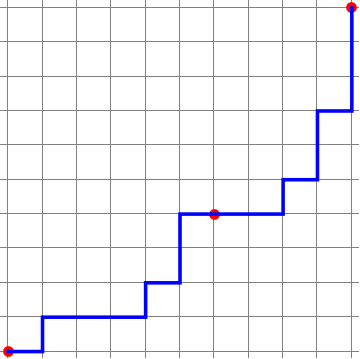
\includegraphics[width=0.9\linewidth]{images/fig-exam-path-1.png}
\caption{Street grid with one path displayed\label{fig-exam-path-1-im}}
\end{figure}
\hypertarget{p-32}{}%
%
\begin{enumerate}
\item\hypertarget{li-8}{}\hypertarget{p-33}{}%
How many paths are there in all from \((0,0)\) to \((10,10)\)?%
\item\hypertarget{li-9}{}\hypertarget{p-34}{}%
How many paths are there that pass through the point \((6,4)\), as does the path in the image?%
\item\hypertarget{li-10}{}\hypertarget{p-35}{}%
One can partition the set of all possible paths from (0,0) to (10,10) according to position of the path after one step. Identify the two points at which you could be at after one step, and then count the number of paths that pass through each of those points.  Write out the sum of these numbers without evaluting them to get an alternative expression for the answer to part (a).%
\end{enumerate}
%
\item\hypertarget{li-11}{}\hypertarget{p-36}{}%
How many different ways can you arrange the letters in the following words. Leave your answers as a product of factorials and other numbers.%
\begin{enumerate}
\item\hypertarget{li-12}{}\hypertarget{p-37}{}%
CHEMISTRY%
\item\hypertarget{li-13}{}\hypertarget{p-38}{}%
MATHEMATICS%
\end{enumerate}
%
\item\hypertarget{li-14}{}\hypertarget{p-39}{}%
Prove either directly or indirectly:  \(p\to \neg q, s\lor p, q \Rightarrow  s\)%
\item\hypertarget{li-15}{}\hypertarget{p-40}{}%
Let \(A=\{1,2,3,4,5\}\). Define relation \(t\)on \(A\) by \(a t b\) if and only if \(b-a\) is even.%
\begin{enumerate}
\item\hypertarget{li-16}{}\hypertarget{p-41}{}%
Draw a digraph of \(t\)%
\item\hypertarget{li-17}{}\hypertarget{p-42}{}%
True or false?: \(t^2= t\).  Explain your answer.%
\end{enumerate}
%
\item\hypertarget{li-18}{}\hypertarget{p-43}{}%
Prove by induction that if \(n\geq 1\),   \(1(1!)+2(2!) +\cdots +n(n!) = (n+1)!-1\)%
\item\hypertarget{li-19}{}\hypertarget{p-44}{}%
Let \(B\) be the set of strings of four bits, \(b_1b_2b_3b_4\) where each bit is either 0 or 1. Define relation \(w\) on \(B\) by \(x w y\) if \(x\) has the same number of 1's as \(y\)%
\begin{enumerate}
\item\hypertarget{li-20}{}\hypertarget{p-45}{}%
Explain why \(w\) is an equivalence relation.%
\item\hypertarget{li-21}{}\hypertarget{p-46}{}%
Into how many equivalence classes is \(B\) divided by \(w\)?%
\item\hypertarget{li-22}{}\hypertarget{p-47}{}%
To what equivalence class does 1000 belong?%
\end{enumerate}
%
\item\hypertarget{li-23}{}\hypertarget{p-48}{}%
Given the following matrices for relations \(r\) and \(s\) on \(\{1,2,3,4,5\}\), determine the matrix for the relation \(r s\). \(R=\left(
\begin{array}{ccccc}
0 & 0 & 1 & 0 & 0 \\
1 & 0 & 0 & 0 & 1 \\
0 & 0 & 0 & 1 & 0 \\
1 & 1 & 0 & 0 & 0 \\
0 & 0 & 1 & 1 & 1 \\
\end{array}
\right)\)  and  \(S=\left(
\begin{array}{ccccc}
0 & 1 & 0 & 0 & 1 \\
0 & 0 & 1 & 0 & 0 \\
0 & 0 & 0 & 0 & 1 \\
1 & 0 & 0 & 0 & 0 \\
0 & 1 & 0 & 0 & 0 \\
\end{array}
\right)\)%
\item\hypertarget{li-24}{}\hypertarget{p-49}{}%
Prove that the set ordered pairs of positive integers is countably infinite. In other words, prove that the set ordered pairs of positive integers, \(\mathbb{P}\times \mathbb{P}\), has the same cardinality as the set of positive integers. Hint: Plot elements \(\mathbb{P}\times
\mathbb{P}\) in the Cartesian plane and use a ``trick'' that was used to show that \(\mathbb{Q}\) is countably infinite.%
\item\hypertarget{li-25}{}\hypertarget{p-50}{}%
Let \(B\) be the set of strings of four bits, \(b_1b_2b_3b_4\), as in an earlier problem. Define two functions, \(f\) and \(g\) on \(B\) by \(f(\)\(b_1b_2b_3b_4\)) = \(b_4b_1b_2b_3\) and \(g\left(b_1b_2b_3b_4\right)= b_4b_3b_2b_1\)%
\begin{enumerate}
\item\hypertarget{li-26}{}\hypertarget{p-51}{}%
Does \(f\) have an inverse? If so, what is it? If not, why?%
\item\hypertarget{li-27}{}\hypertarget{p-52}{}%
Does \(g\) have an inverse? If so, what is it? If not, why?%
\item\hypertarget{li-28}{}\hypertarget{p-53}{}%
Are the two functions \(f\circ g\) and \(g\circ f\) equal? Explain your answer.%
\end{enumerate}
%
\item\hypertarget{li-29}{}\hypertarget{p-54}{}%
Determine a closed form expression for the sequence \(T\) such that \textbackslash{}\textbackslash{} \(T(n) -2T(n-1)-15T(n-2)=16\)   with  \(T(0)=5\) and \(T(1)=10\)%
\item\hypertarget{li-30}{}\hypertarget{p-55}{}%
I'm thinking of a number between 1 and 1 million.  For every guess you make at my number, I'll tell you whether your guess is too high or too low.   How many guesses would you need if you use a binary search?  Hint:  One million is slightly less than \(2^{20}\).%
\end{enumerate}
%
\end{sectionptx}
%
%
\typeout{************************************************}
\typeout{Section 2.2 Group Theory Exam (2 hours)}
\typeout{************************************************}
%
\begin{sectionptx}{Group Theory Exam (2 hours)}{}{Group Theory Exam (2 hours)}{}{}{im-2h-11-15}
\begin{introduction}{}%
\hypertarget{p-56}{}%
This exam tests students primarily on the topics in Chapters 11 and 15.%
\end{introduction}%
\hypertarget{p-57}{}%
\leavevmode%
\begin{enumerate}
\item\hypertarget{li-31}{}\hypertarget{p-58}{}%
Let \(S\) be a nonempty set and \(*\) a binary operation on \(S\). Clearly and precisely state the conditions that are necessary \([S,*]\) to be a group.%
\item\hypertarget{li-32}{}\hypertarget{p-59}{}%
Let \(A\) be a nonempty set and \(\mathcal{P}(A)\) the set of all subsets of \(A\).%
\begin{enumerate}
\item\hypertarget{li-33}{}\hypertarget{p-60}{}%
What is the identity for intersection on \(\mathcal{P}(A)\)?%
\item\hypertarget{li-34}{}\hypertarget{p-61}{}%
For what sets \(X \in \mathcal{P}(A)\) is there an inverse with respect to intersection?%
\end{enumerate}
%
\item\hypertarget{li-35}{}\hypertarget{p-62}{}%
%
\begin{enumerate}
\item\hypertarget{li-36}{}\hypertarget{p-63}{}%
Find integers \(x\) and \(y\) such that \(101x + 33 y = \gcd (101,33)\)%
\item\hypertarget{li-37}{}\hypertarget{p-64}{}%
What are the additive and multiplicative inverses of 33 for modular addition and multiplication modulo 101?%
\end{enumerate}
%
\item\hypertarget{li-38}{}\hypertarget{p-65}{}%
List the elements that are in the cyclic subgroup generated by 5 in the multiplicative group of units mod 13, \(U_{13}\).%
\item\hypertarget{li-39}{}\hypertarget{p-66}{}%
Define the \emph{direct product} of two groups \(\left[G_1; *_1\right]\) and \(\left[G; *_2\right]\) by clearly identifying the elements and operation of this group.%
\item\hypertarget{li-40}{}\hypertarget{p-67}{}%
Suppose elements of \(\mathbb{Z}_{29}\) are encrypted using the function \(f:\mathbb{Z}_{23}\to \mathbb{Z}_{23}\) such \(f(i)=7i +12 \pmod{23}\).%
\begin{enumerate}
\item\hypertarget{li-41}{}\hypertarget{p-68}{}%
Find a formula for the inverse of \(f\).%
\item\hypertarget{li-42}{}\hypertarget{p-69}{}%
Find the value of \(k\) such that \(f(k)=2\).%
\end{enumerate}
%
\item\hypertarget{li-43}{}\hypertarget{p-70}{}%
Prove that \(f:\mathbb{R}^+\to  \mathbb{Z}\) defined by \(f(x)=\log_{2}x\) is an isomorphism from \(\left[\mathbb{R}^+;\cdot \right]\) \textbraceleft{} \textbraceright{}into \([\mathbb{R};+]\).%
\item\hypertarget{li-44}{}\hypertarget{p-71}{}%
Find the least nonnegative integer, \(x\), such that \(x\equiv 11\pmod{19}\) and \(x \equiv 1 \pmod{16}\).%
\item\hypertarget{li-45}{}%
\begin{enumerate}
\item\hypertarget{li-46}{}\hypertarget{p-72}{}%
List all left cosets, without duplication, of the cyclic subgroup of \(\mathbb{Z}_{15}\) generated by 10, \(\langle $10$\rangle\)%
\item\hypertarget{li-47}{}\hypertarget{p-73}{}%
What group is \(\left.\mathbb{Z}_{15}\right/\langle 10\rangle\) isomorphic to?%
\end{enumerate}
%
\item\hypertarget{li-48}{}\hypertarget{p-74}{}%
Let \([G,*]\) be a group, \(H\) a subgroup of \(G\), and \(a, b\in G\). Prove that \(b \in  a*H\) if and only if \(a^{-1}*b \in H\).%
\item\hypertarget{li-49}{}\hypertarget{p-75}{}%
Let \(r=(1,2,3,4,5,6,7)\) and \(f=(1,7)(2,6)(3,5)\) be elements of the group \(S_7\).%
\begin{enumerate}
\item\hypertarget{li-50}{}\hypertarget{p-76}{}%
What is the orders of \(r\) and \(f\)?%
\item\hypertarget{li-51}{}\hypertarget{p-77}{}%
Compute \(f^{-1}\) , \(r\circ f\) and \(f^{-1}\circ r\circ f\).%
\item\hypertarget{li-52}{}\hypertarget{p-78}{}%
Are \(r\) and \(f\) odd or even?%
\item\hypertarget{li-53}{}\hypertarget{p-79}{}%
Is the cyclic subgroup of \(S_7\) generated by \textbackslash{}textit\textbraceleft{} r\textbraceright{} a normal subgroup?  Explain your answer.%
\end{enumerate}
%
\item\hypertarget{li-54}{}\hypertarget{p-80}{}%
Consider the linear code defined by the function \(E:\mathbb{Z}_2{}^3\to \mathbb{Z}_2{}^6\) where \(E(a)= a G\) and%
\begin{equation*}
G=\left(
\begin{array}{cccccc}
1 & 0 & 0 & 1 & 1 & 0 \\
0 & 1 & 0 & 0 & 0 & 1 \\
0 & 0 & 1 & 0 & 1 & 1 \\
\end{array}
\right)\text{.}
\end{equation*}
%
\begin{enumerate}
\item\hypertarget{li-55}{}\hypertarget{p-81}{}%
What is the range of \(E\) called?%
\item\hypertarget{li-56}{}\hypertarget{p-82}{}%
Determine a parity check matrix based this code.%
\item\hypertarget{li-57}{}\hypertarget{p-83}{}%
Can this code be used to detect single bit errors? Can it be used to correct all single bit errors? If not, are there any errors that it can correct?%
\end{enumerate}
%
\end{enumerate}
%
\end{sectionptx}
\end{chapterptx}
%
\backmatter
%
%
%% A lineskip in table of contents as transition to appendices, backmatter
\addtocontents{toc}{\vspace{\normalbaselineskip}}
%
%
%
\typeout{************************************************}
\typeout{References  References}
\typeout{************************************************}
%
\begin{references-chapter-numberless}{References}{}{References}{}{}{references-1}
\index{References}\begin{introduction}{}%
\hypertarget{p-84}{}%
This is a list of recommendations for discrete mathematics courses that have been issued by various professional organizations.%
\end{introduction}%
%% If this is a top-level references
%%   you can replace with "thebibliography" environment
\begin{referencelist}
\bibitem[1]{im-biblio-dossey-1990}\hypertarget{im-biblio-dossey-1990}{}Dossey, John A., \textit{Discrete Mathematics: The Math For Our Time.” In Discrete Mathematics Across the Curriculum K-12},1990 Yearbook of the National Council of Teachers of Mathematics, edited by Margaret J. Kenney and Christian R. Hirsch. Reston, Va.: NCTM, 1990
\bibitem[2]{im-biblio-maa-1986}\hypertarget{im-biblio-maa-1986}{}Mathematical Association of America (MAA), \textit{Report of the Committee on Discrete Mathematics in the First Two Years}, Washington, D. C.: MAA, 1986
\bibitem[3]{im-biblio-nctm-1990}\hypertarget{im-biblio-nctm-1990}{}National Council of Teachers of Mathematics (NCTM), \textit{Discrete Mathematics and the Secondary Mathematics Curriculum}, Reston, Va.: NCTM, 1990
\end{referencelist}
\end{references-chapter-numberless}
\end{document}